%%==================================================
%% chapter04.tex for BIT Master Thesis
%% modified by yang yating
%% version: 0.1
%% last update: Dec 25th, 2016

%% modified by Meng Chao
%% version: 0.2
%% last update: May 29th, 2017
%%==================================================
\chapter{基于特征的单目半稠密SLAM算法}
\label{chap:Semi-Dense}

针对第三章提到的基于特征的单目SLAM算法构建地图稀疏,无法用于导航和后续任务规划的问题,本章研究改进基于特征的单目SLAM算法,在原有基于特征的ORB-SLAM算法的基础上,参考直接法SLAM半稠密地图构建的原理,构建环境的半稠密地图。不同于直接法SLAM中使用多帧连续帧对参考帧逆深度进行滤波的方法,本文使用经过局部BA(local BA)和位姿图(pose graph)优化后的关键帧进行重构,可获得较高精度的定位和地图重构效果。改进的基于特征的单目SLAM算法主要包括5个部分,立体搜索约束,极线搜索和块匹配,逆深度假设融合,帧内逆深度假设一致性检验和帧间逆深度假设一致性检验,其算法流程图如图\ref{fig4.1}所示,具体算法流程如下:
\begin{enumerate}[label={(\arabic*)}]

\item 对选取的关键帧$K_i$,提取图像中像素灰度梯度满足阈值的像素点,在临近的$N$个关键帧中进行极线搜索,得到像素的逆深度假设。

\item 考虑到图像在观测过程中存在噪声、视差过小和二义性等问题,假设逆深度服从高斯分布,并且认为相机关键帧的位姿是准确的,不考虑位姿的不确定性。

\item 由于关键帧之间的极线搜索是在宽基线条件下进行,搜索范围较大,需要考虑匹配过程中的误匹配。除考虑更多像素匹配约束外,采用高斯分布表示逆深度图中像素$p$的逆深度假设$N(\rho_p, \sigma_{\rho_p}^2)$,通过融合一致的逆深度假设降低误匹配的影响。

\item 对关键帧逆深度图中的像素逆深度进行融合,并且通过帧内逆深度假设一致性检验剔除与临近像素逆深度不一致的像素。

\item 完成当前关键帧和其相邻关键帧的逆深度假设计算后,对其当前帧和相邻帧的像素逆深度进行一致性检验,剔除不一致的像素逆深度,并通过最小化深度误差函数优化像素深度。

\end{enumerate}

本文改进的基于特征的单目SLAM算法是在宽基线条件下进行的关键帧间极线搜索,宽基线的极线搜索容易导致误匹配和离群值影响重构效果。因而相比于基于直接法的半稠密SLAM算法,为了提高本算法的鲁棒性,进行极线搜索时除考虑灰度梯度大小和方向的匹配性外,还应进行逆深度假设融合和帧内与帧间逆深度假设一致性检验,剔除宽基线极线搜索的误匹配点,从而提升重构效果。

%4.1 半稠密ORB SLAM重构流程
\begin{figure}
\centering
%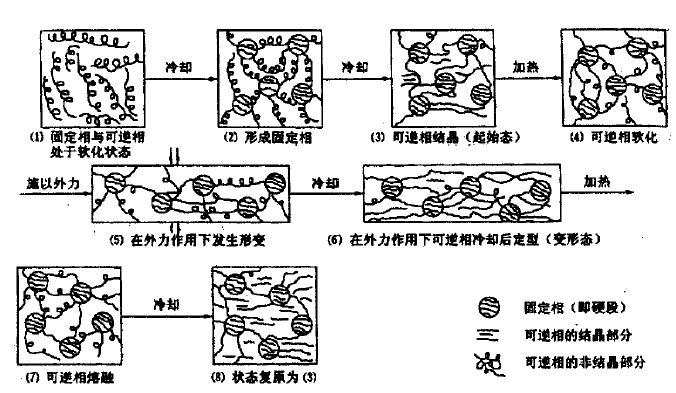
\includegraphics[width=0.75\textwidth]{figures/figure1}
\caption{基于特征的半稠密单目SLAM算法流程图}
\label{fig4.1}
\end{figure}





% 4.1
\section{立体搜索约束}
本章改进的基于特征的单目SLAM算法可以提供相机位姿$R,t$, 用于像素对应匹配点的搜索进而得到像素逆深度假设。由于已知当前关键帧ORB特征点的深度信息,可以估计当前关键帧的最大逆深度$\rho_{max}$, 最小逆深度$\rho_{min}$和像素逆深度的先验信息$N\left( \rho_0,\sigma_{\rho_0}^2  \right)$,其中$\rho_{max}=\rho_0+2\sigma_{\rho_0}$,$\rho_{min}=\rho_0-2\sigma_{\rho_0}$。另外,通过Covisibility图可以获得与当前关键帧$K_i$具有最多共视关系的前$N$个关键帧的集合$K$,从而完成关键帧间的立体搜索。通过立体搜索约束求解当前关键帧的逆深度假设时,应在关键帧插入之后一个帧率的时间内不处理新插入关键帧。一方面可以避免由于局部BA导致的共视图结构变化;另一方面可以引入当前关键帧之后的关键帧,提高重建效果。


%4.2
\section{极线搜索与块匹配}
对于当前关键帧$K_i$中像素梯度的模大于$\lambda_G$的像素$p$,会在关键帧$K_j \in K$的极线$l_j$上$\left[ \rho_{min}, \rho_{max} \right]$范围内进行搜索,寻找匹配的像素点,如图\ref{fig4.2}所示。极线利用基本矩阵$F_{ji}$求得,极线搜索方程如下所示。
\begin{equation}
\label{equ4.1}
x_j^T F_{ji}x_p = x^T_jl_j=0 \rightarrow v_j = m \cdot u_j+n
\end{equation}

\begin{figure}
\centering
%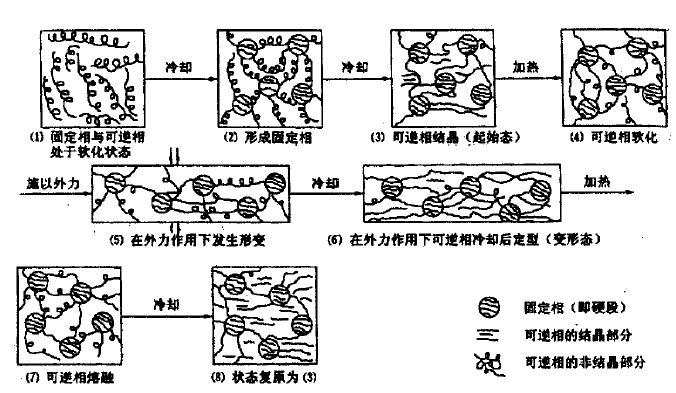
\includegraphics[width=0.75\textwidth]{figures/figure1}
\caption{极线搜索}
\label{fig4.2}
\end{figure}

不同于直接法SLAM中的窄极线匹配,本章的改进算法极线搜索是在宽基线条件下进行的,因而除了区块匹配外,需要加入更多约束。除了比较像素灰度$I$之外,还需要比较像素的梯度模$G$和梯度方向$\Uptheta$,从而在极线$l_j$上找到合适的像素匹配。根据以下设计约束, 排除$l_j$极线上不满足条件的像素。


\begin{enumerate}[label={(\arabic*)}]

\item 属于关键帧$K_j \in K$上的像素$p_j$必须在图像中像素梯度大的区域,像素梯度应大于阈值,$G(u_j)> \lambda_G$。

\item 考虑到匹配的二义性与沿极线方向的像素梯度有关,因而像素梯度方向不能与极线方向垂直,满足$\vert \Uptheta(u_j)-\Uptheta_L \pm \pi \vert < \lambda_L$,其中$\Uptheta_L$表示基线方向。

\item 图像的匹配像素$p_j$与$p_i$的梯度方向应该相近,满足$\vert \Uptheta(u_j)-(\Uptheta_L \pm \Delta \theta_{j,i} \vert < \lambda_\theta $,其中$\Delta \theta_{j,i}$表示两帧图像之间的旋转角度。

\end{enumerate}
以上区块匹配约束可以剔除关键帧$K_j \in K$极线上$l_j$的大部分像素点,剩余的为关键帧$K_i$中的像素$p$可能的匹配点。为了比较两个像素点的相似性, 定义像素相似误差函数$e(u_j)$:
\begin{equation}
\label{equ4.2}
\begin{aligned}
& e(u_j) = {r_I^2 \over \sigma_I^2} + {r_G^2 \over \sigma_G^2} \\ 
& r_I = I_p-I(u_j),\  r_G = G_p-G(u_j)
\end{aligned}
\end{equation}
其中$r_I$和$r_G$表示像素灰度和梯度误差,$\sigma_I$和$\sigma_G$表示像素灰度和梯度的标准差。由于像素梯度是根据像素的灰度计算得到,若利用施密特算子$\triangledown$计算梯度, 则像素灰度与梯度的误差具有相性,
$\sigma_G^2=\theta \sigma_I^2$ , $ \theta = 0.23$。公式\eqref{equ4.2}可以简化为
\begin{equation}
\label{equ4.3}
 e(u_j) = \left( {r_I^2}+{1 \over \theta} r_G^2 \right) {1 \over \sigma_I^2}
\end{equation} 

相似误差函数最小化的坐标$u_0$表示的像素为对应的匹配像素, 其灰度误差和梯度误差为$r_{I_0}$,$r_{G_0}$,误差函数导数为
\begin{equation}
\label{equ4.4}
{\partial e \over \partial u_j } = -{ -2(r_I g+ { 1 \over \theta} r_G q )  \over \sigma_I^2 }
\end{equation}
令其中$g$是灰度梯度的模,$q$是灰度梯度导数的模,方向与极线相同。
\begin{equation}
\label{equ4.5}
\begin{aligned}
& g \approx { {I(u_j+1) - I(u_j-1)} \over 2 } \\
& q \approx { {G(u_j+1) - G(u_j-1)} \over 2 } 
\end{aligned}
\end{equation}

令公式\eqref{equ4.4}等于$0$可以得到匹配的像素坐标$u_0$,实际情况下像素坐标$u_0$是沿极线以像素为步长搜索得到的整数坐标,而公式\eqref{equ4.4}的解不一定是整数。设真值为$u_0^*=u_0+\Delta u$,对方程\eqref{equ4.2}中的误差进行一阶泰勒近似,带入导数等于$0$的公式\eqref{equ4.4}中可以得到
\begin{equation}
\label{equ4.6}
\Delta u = {{ r_I(u_0) g(u_0)+ {1 \over \theta} r_G(u_0)q(u_0) } \over {g^2(u_0)+ { 1 \over \theta} q^2(u_0)}}
\end{equation}
匹配像素的亚像素精度坐标为
\begin{equation}
\label{equ4.7}
u_0^* = u_0 + {{ r_I(u_0) g(u_0)+ {1 \over \theta} r_G(u_0)q(u_0) } \over {g^2(u_0)+ { 1 \over \theta} q^2(u_0)}}
\end{equation}

根据误差传递理论,通过像素灰度的方差$\sigma_I^2$可以得到匹配像素坐标$u_0^*$的不确定性。
\begin{equation}
\label{equ4.8}
\sigma_{u_0^*}^2 = \left \vert { \partial u^* \over \partial r_I(u_0) }  \right \vert \sigma_I^2 + \left \vert { \partial u^* \over \partial r_G(u_0) }  \right \vert \sigma_G^2 = { \sigma_I^2 \over g^2(u_0) + {1 \over \theta} q^2(u_0) }
\end{equation}
根据像素坐标不确定性可以知道,沿极线方向像素灰度梯度和像素灰度梯度导数的模越大,匹配的可靠性越高。

为了得到匹配像素的逆深度假设不确定性,需要计算当前关键帧$K_i$中像素$p$的逆深度$\rho_p$。根据地图点云的三角化公式$s_jX_j = s_pR_{ji}X_p+t_{ji}, \  X_j = K^{-1}P_j, X_p = K^{-1}P_p$,可以得到像素逆深度为
\begin{equation}
\label{equ4.9}
\rho_p(u_j) = { r_z^{ji} X_p (u_j-c_x) - f_x r_x^{ji} X_p  \over - t_z^{ji}(u_j-c_x)+f_x t_x^{ji} }
\end{equation}
其中$r_x^{ji}$,$r_z^{ji}$表示两帧间的旋转矩阵$R_{ji}$的第一行和第三行,$t_x^{ji}$,$t_z^{ji}$表示来两帧间的平移向量$t_{ji}$的第一个和第三个元素;$f_x$,$c_x$是相机内参;$\rho_p = { 1 \over s_p}$,$P_j= \left [ u_j, v_j, 1 \right ] ^T$,利用方程\eqref{equ4.9}可以得到像素$p_i$与像素$p_j$对应的逆深度假设$N(\rho_j, \sigma_{\rho_j}^2)$。
\begin{equation}
\label{equ4.10}
\begin{aligned}
 \rho_j &= \rho_p(u_0^*) \\ 
 \sigma_{\rho_j} &= max \left( \left \vert  \rho_p(u_0^*+\sigma_{u_0^*})-\rho_j \right \vert , \  \left \vert  \rho_p(u_0^*-\sigma_{u_0^*})-\rho_j \right \vert \right)
\end{aligned}
\end{equation}

在以上的逆深度假设推导过程中,并没有像直接法SLAM一样引入帧间小旋转运动假设,因而本算法的逆深度假设不确定性具有一般性。


%4.3
\section{逆深度假设融合}
根据之前4.2节中介绍的方法,每个像素可以得到一组逆深度假设。由于存在极线上的像素逆深度立体搜索约束,且极线上匹配的像素需满足之前提到的像素梯度约束,因而逆深度假设的个数可能不足$N$个。另外,由于像素的相似性和遮挡,以上逆深度假设中存在离群值。为了验证像素逆深度假设,在像素对应的一组逆深度假设中至少应该找到$\lambda_N$个一致假设。利用$\chi^2$假设检验(置信区间$95\%$,自由度2),验证两个逆深度假设分布的一致性。
\begin{equation}
\label{equ4.11}
{ (\rho_a - \rho_b)^2 \over \sigma_a^2 }+{ (\rho_b - \rho_a)^2 \over \sigma_b^2} < 5.991
\end{equation}

每次从一组像素的逆深度假设中选取一个,与其他逆深度假设进行一致性检验,若与其一致的逆深度假设数量超过$\lambda_N$个,则对该组逆深度按照公式\eqref{equ4.12}进行融合,像素$p$融合后的逆深度假设服从$N(\rho_p,\sigma_{\rho_p}^2)$,其中$n$表示通过检验的逆深度假设数量。
\begin{equation}
\label{equ4.12}
\rho_p = { {\sum\limits_n {1 \over \sigma_{\rho_j}^2} \rho_j } \over \sum\limits_n {1 \over \sigma_{\rho_j}^2}  }, \ 
\sigma_{\rho_p}^2 = {1 \over  \sum\limits_n { 1 \over \sigma_{\rho_j}^2}  }
\end{equation}


%4.4
\section{帧内逆深度假设一致性检验}
在完成当前关键帧$K_i$中像素的逆深度假设计算和融合后,需要对帧内所有逆深度假设进行一致性检验,用于剔除像素逆深度假设中的离群值。首先,通过公式\eqref{equ4.11}检验某像素和它临近的8个像素点的逆深度假设的一致性,若一致的逆深度假设数量大于2,则保留该像素点的逆深度假设,否则剔除该点逆深度假设。若保留该像素,其逆深度根据公式\eqref{equ4.12}进行融合,不确定性为所有参与逆深度假设检验的像素中的最小不确定性。对于处于像素灰度变化明显区域但没有逆深度假设的像素点,若在该像素周围至少有两个逆深度假设一致的像素,则给该像素点添加逆深度假设,逆深度为附近一致逆深度假设的逆深度均值,不确定性是附近一致逆深度假设中的最小值,该方法可以增加地图重建的稠密性,起到平滑地图的作用。

%4.5
\section{帧间逆深度假设一致性检验}
在当前关键帧$K_i$的$N$个临近关键帧的逆深度地图全部计算完成后,对关键帧$K_i$中像素的逆深度假设进行帧间一致性检验。对于关键帧$K_i$中的像素$p$对应的逆深度$\rho_p$,将其投影到$K_i$临近的关键帧$K_j \in K$中,并计算像素$p$在关键帧$K_j \in K$中对应点的逆深度:
\begin{equation}
\label{equ4.13}
\begin{aligned}
& x_j = K R_{ji} {1 \over \rho_p} X_p + Kt_{ji} \\ 
& \rho_j = { \rho_p \over r_z^{ji}X_p+\rho_p t_z^{ji} }
\end{aligned}
\end{equation}
其中$x_{j}$表示关键帧$K_i$中的像素$p$在$K_j \in K$中对应点的像素坐标。若$x_j$不是证书像素坐标,搜索$x_{j}$临近的4个像素,通过$\chi^2$假设检验(置信区间$95\%$,自由度$1$),检验是否与$x_j$逆深度假设一致。
\begin{equation}
\label{equ4.14}
{ (\rho_j - \rho_{j,n})^2 \over \sigma_{\rho_{j,n}}^2 } < 3.84
\end{equation}

如果在$\rho_{j,n}$中存在与$x_j$逆深度假设一致的像素点,则可以保留像素点$x_j$的逆深度假设。如果在当前关键帧$K_i$的$N$个临近关键帧中至少有$\lambda_N$个关键帧可以找到像素p的对应像素点$x_j$的逆深度假设,则保留当前关键帧$K_i$中像素$p$的逆深度假设。

最后对关键帧像素进行重投影,以深度$d_p = { 1 \over \rho_p }$为优化变量,利用公式\eqref{equ4.15}通过高斯-牛顿方法最小化深度误差函数,优化像素点的逆深度,提高重构精度。
\begin{equation}
\label{equ4.15}
d_p^* = \min_{d_p} \sum\limits_{j,n} \left( d_{j,n} - d_p r_z^{ji} X_p - t_z^{ji}  \right)^2  {1 \over {d_{j,n}^4 \sigma_{\rho_{j,n}}^2 }}
\end{equation}
优化的目标函数选择深度作为优化变量而不是逆深度,是因为从方程\eqref{equ4.13}中可以发现,以深度作为变量时,深度误差函数是线性的。并考虑深度对应的不确定,不同深度置信度在总误差的权重不同,优化更为精确。




\section{本章小结}

采取了什么方法,针对出现的问题进行优化,表现出了比现有算法更好的性能。







\iffalse
We evaluate the LSD algorithm hand holding camera in indoor environment. We test two time for the different sample key frames. The result is show in Fig.4 The picture (a) and (b) are the reference image and the key frame. The (c) and (d) are the reconstruction 3D map of the LSD-SLAM. The result is expressed the more key frames can be get the more detail of the environment, now that the noisy of the environment will affect the performance of LSD.

\begin{figure}
    \centering
       %\begin{minipage}{5cm}
       	  \subfigure[]
       	  {
          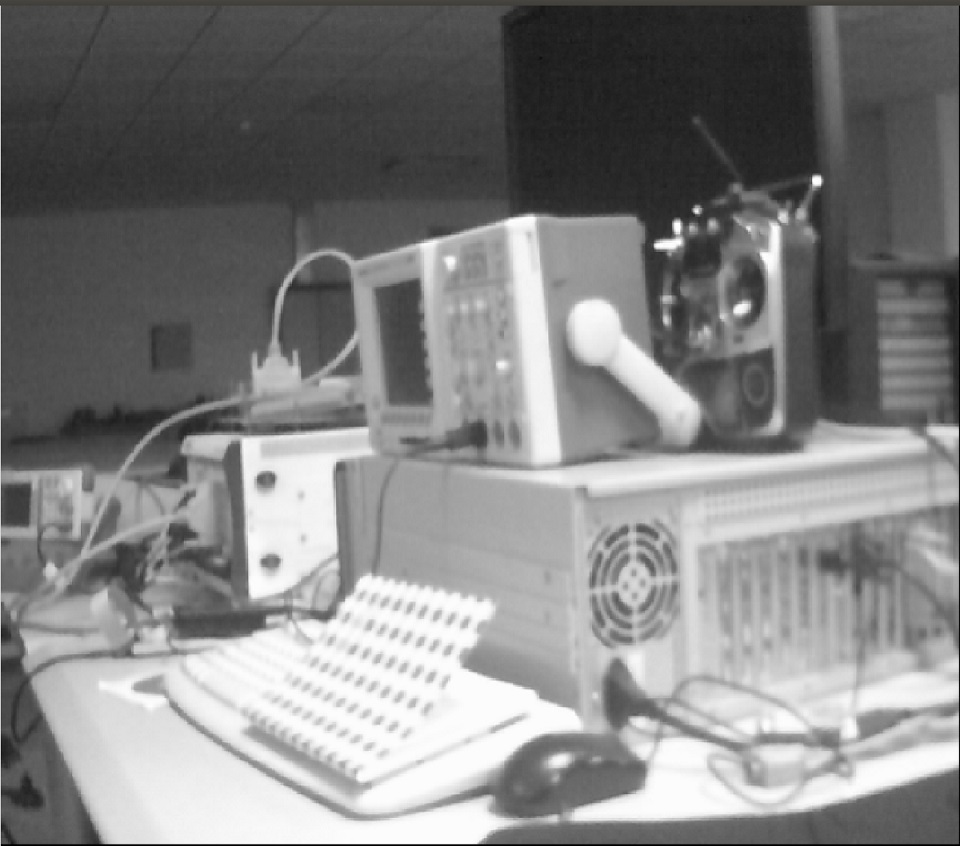
\includegraphics[scale=.2]{figures/Fig4(a)}          
          %\subcaption{}
          }                    
          \subfigure[]
       	  {
          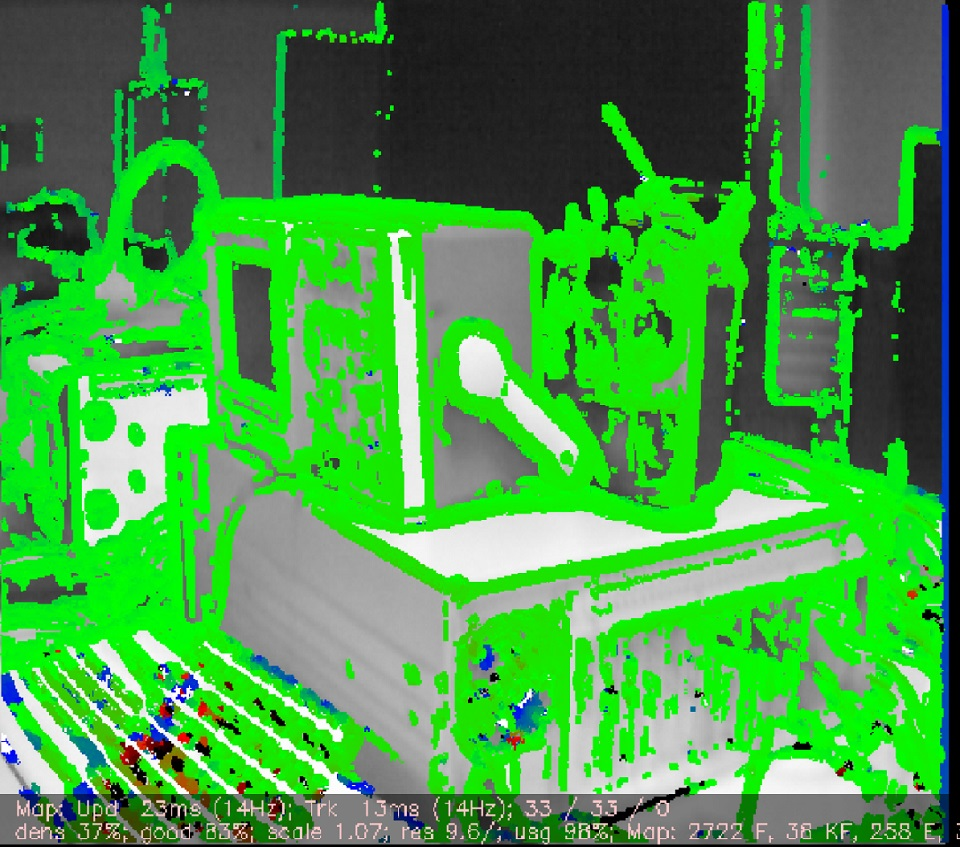
\includegraphics[scale=.2]{figures/Fig4(b)}
          %\subcaption{}
          }
          \hspace{0in}
     
          \subfigure[]
       	  {
          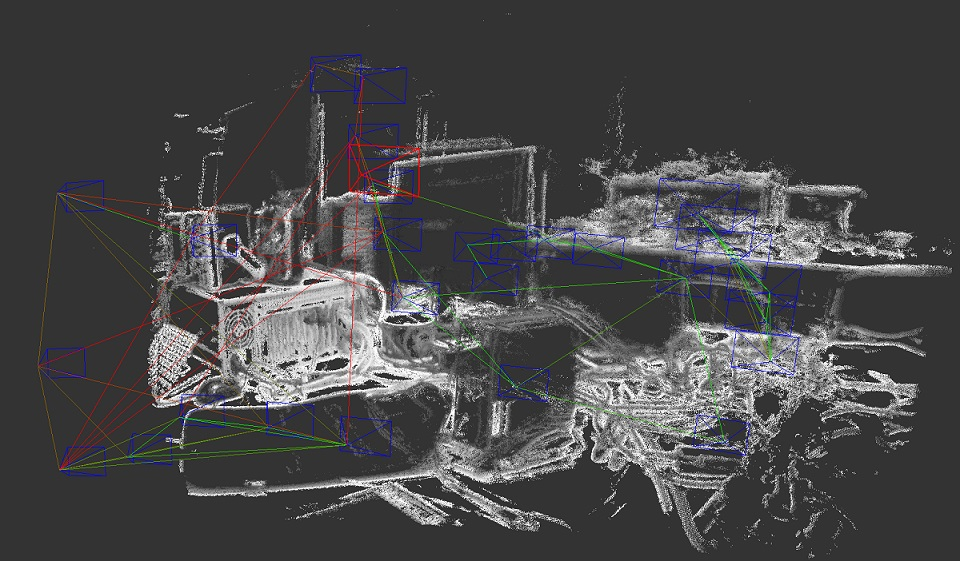
\includegraphics[scale=.25]{figures/Fig4(c)}
          %\subcaption{}
		  }
		  \subfigure[]
       	  {          
          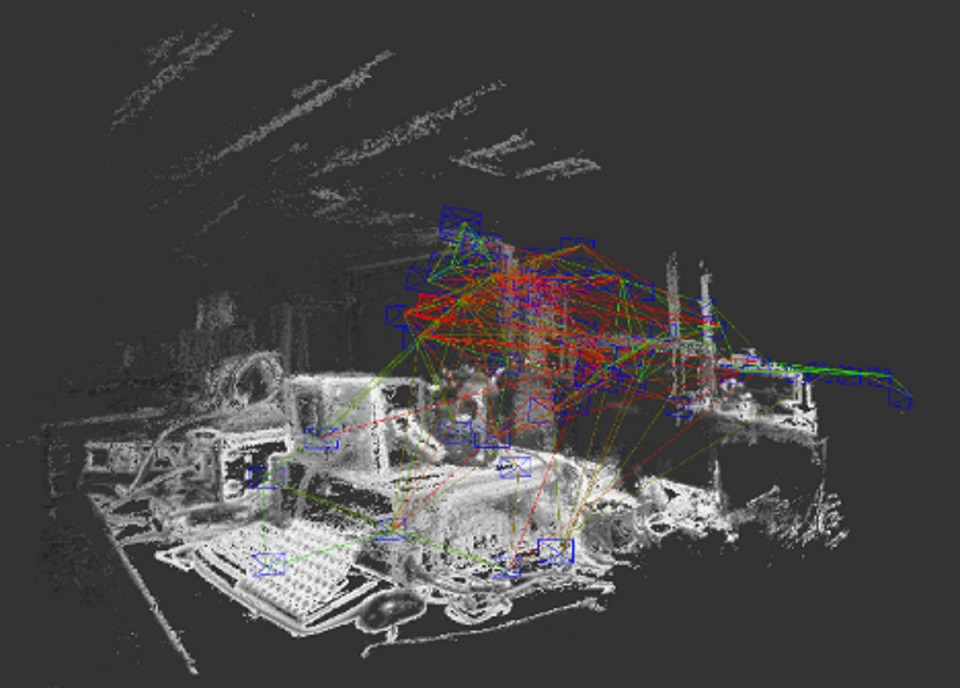
\includegraphics[scale=.2]{figures/Fig4(d)}
          %\subcaption{}
          }
          \hspace{0in}
       %\end{minipage}
     \caption{The indoor LSD-SLAM Map}
\end{figure}

\fi



\iffalse
We evaluate the LSD-SLAM performance in outdoor. We accomplish the reconstruction the 3D map in diverse scene which is different distance. The result is expressed in Fig.5

The picture (a) and (b) are the different distance scene reference image for hand holding camera. The (c) and (d) is the reconstruction map of the LSD-SLAM. We can find that the mapping is completely reconstructed the scene information and the noisy is low in outdoor environment. This can be used in unmanned aerial vehicle(UAV) navigation and localization. The LSD-SLAM is reliable and robustness.

\begin{figure}
    \centering
       %\begin{minipage}{5cm}
       	  \subfigure[]
       	  {
          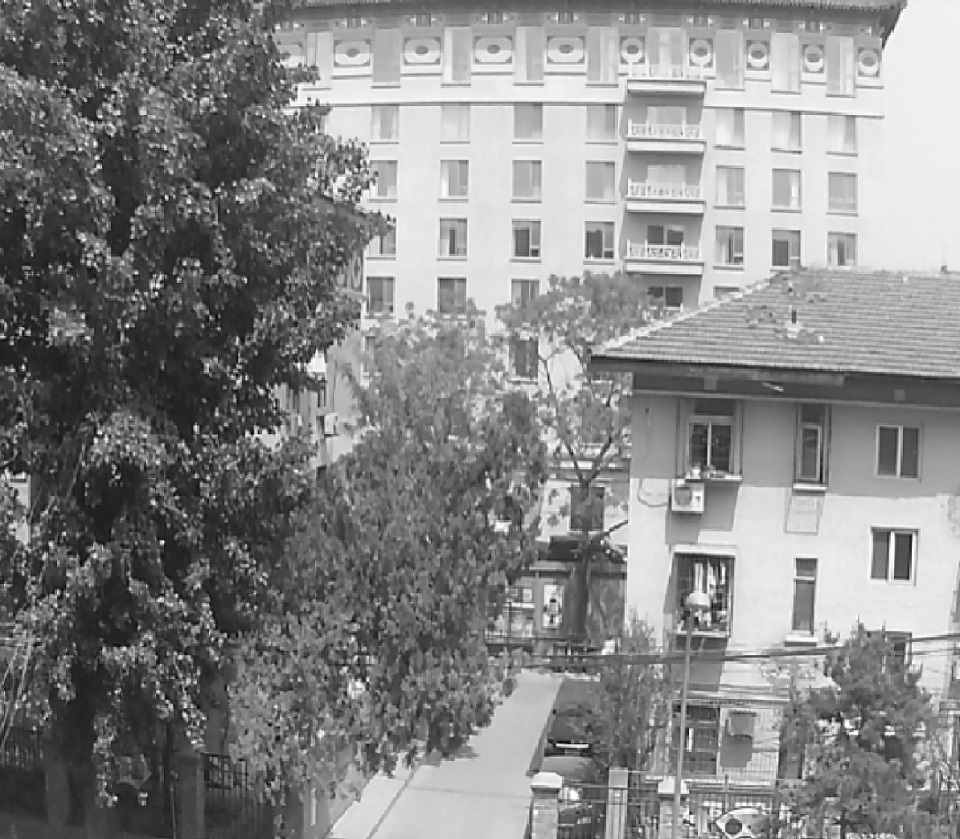
\includegraphics[scale=.2]{figures/Fig5(a)}          
          %\subcaption{}
          }                    
          \subfigure[]
       	  {
          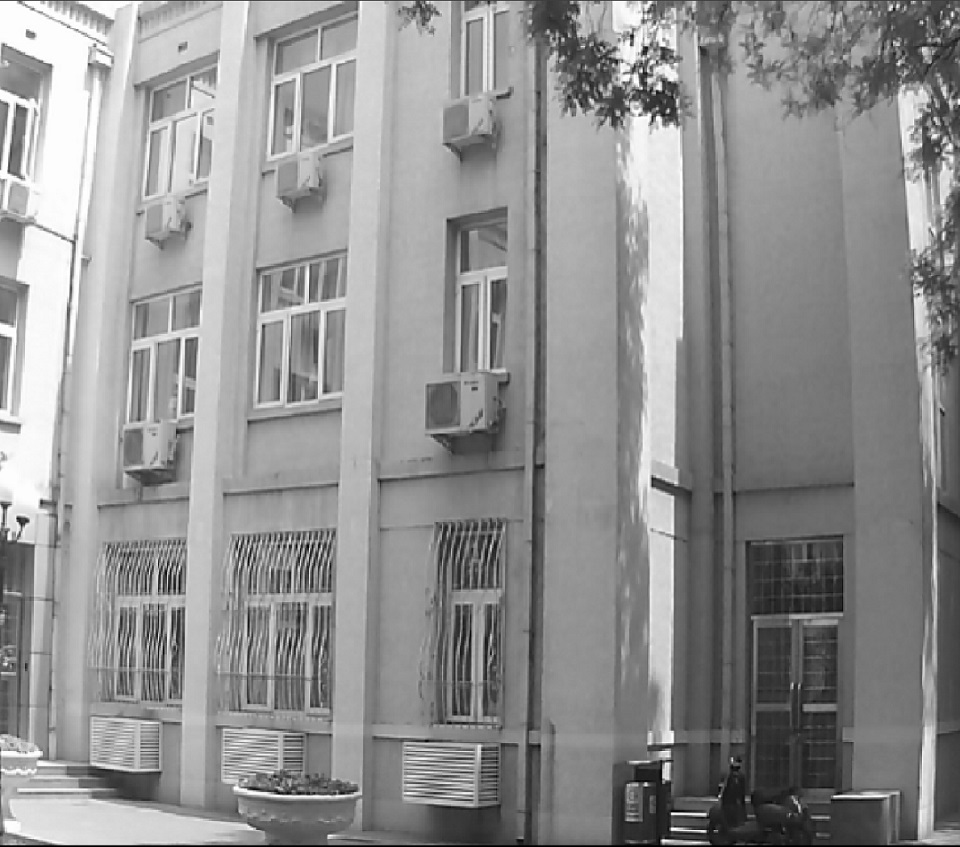
\includegraphics[scale=.2]{figures/Fig5(b)}
          %\subcaption{}
          }
          \hspace{0in}
     
          \subfigure[]
       	  {
          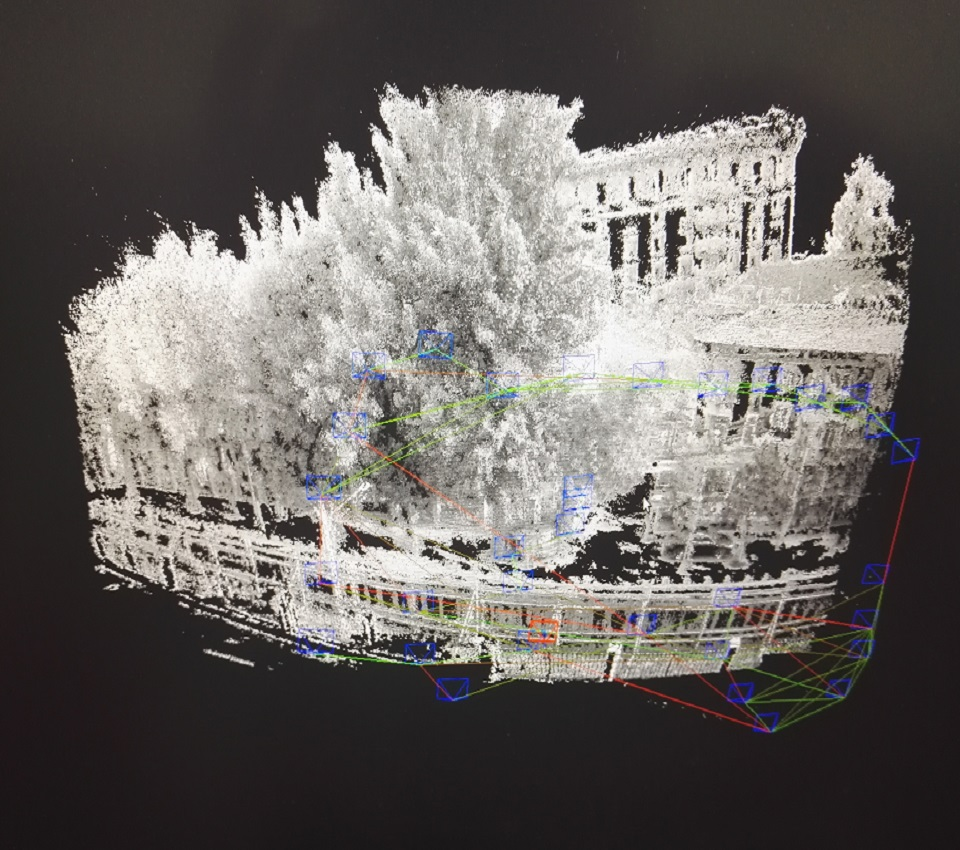
\includegraphics[scale=.25]{figures/Fig5(c)}
          %\subcaption{}
		  }
		  \subfigure[]
       	  {          
          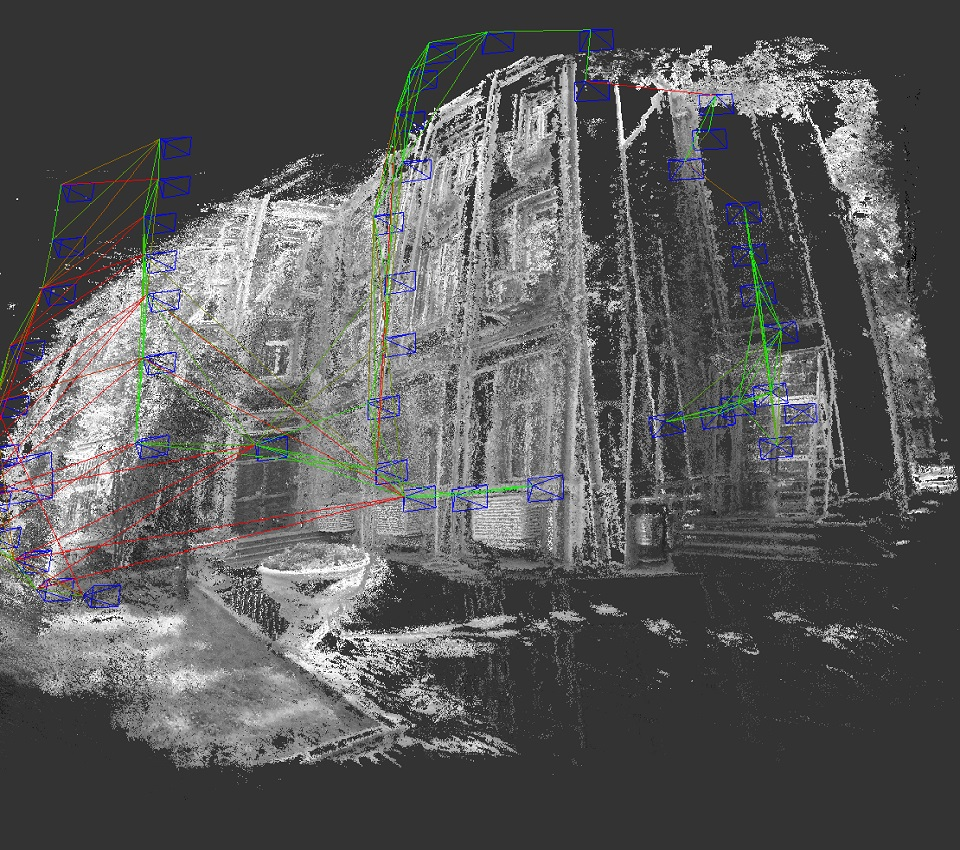
\includegraphics[scale=.2]{figures/Fig5(d)}
          %\subcaption{}
          }
          \hspace{0in}
       %\end{minipage}
     \caption{The outdoor LSD-SLAM Map}
\end{figure}
\fi




\iffalse
\begin{table}
\newcommand{\tabincell}[2]{\begin{tabular}{@{}#1@{}}#2\end{tabular}}
\centering

    \caption{Localization Error in Tum Dataset}     % NOTE!  caption goes _before_ the table contents !!
    
	\renewcommand\arraystretch{1.5}
    \begin{small}
    \begin{tabular}{p{2cm}p{1.5cm}p{1.5cm}p{1.5cm}}
    \hline

    \multicolumn{1}{c}{\multirow{3}{*}{Seq.}}
    & \multicolumn{3} {c} {\bfseries\tabincell{c} {Absolute Key Frame \\ Trajectory RMSE(cm)}} \\
    \cline{2-4}
    \multicolumn{1}{c}{}&   \multicolumn{1}{c}{\bfseries \tabincell{c}{LSD-SLAM} }      &     \multicolumn{1}{c}{\bfseries \tabincell{c}{ semi-dense \\mono-VO}}   & \multicolumn{1}{c}{\bfseries \tabincell{c}{ RGB-D \\SLAM}} \\	

    \cline{1-4}


  \multicolumn{1}{c}{fr2/desk}     &\multicolumn{1}{c}{5.65}      &\multicolumn{1}{c}{13.50}       &\multicolumn{1}{c}{2.58}   \\

  \multicolumn{1}{c}{Fr2/xyz}       &\multicolumn{1}{c}{2.15}      &\multicolumn{1}{c}{3.79}        &\multicolumn{1}{c}{1.34}   \\

  \multicolumn{1}{c}{sim/slowmo}    &\multicolumn{1}{c}{0.37}      &\multicolumn{1}{c}{2.21}        &\multicolumn{1}{c}{0.13}   \\

  \hline

    \end{tabular}
    \end{small}
\end{table}

The LSD-SLAM is evaluated on the Tum dataset. It is very challenging because of containing fast rotational movement, strong motion blur and rolling shutter artifacts. The result is displayed in tableⅠand compared with other algorithm for the localization accuracy.We use the very first depth map to bootstrap the system and get the correct initial scale.

\fi